\section{Stima dei parametri del sistema nel mondo reale}
Non tutti i parametri descritti in tabella \ref{tab:parametri} sono calcolabili facilmente. In particolare, mi sono sconosciuti:
\begin{itemize}
    \item I parametri del motore.
    \item Il momento d'inerzia del pendolo.
\end{itemize}
In questa sezione userò i dati raccolti dal sistema reale per ottenere una stima di questi parametri.
Anche qui, mi conviene separare lo studio del pendolo dallo studio del motore.

\subsection{Parametri del pendolo}
La massa del pendolo si può misurare direttamente con una bilancia.
Anche la posizione del centro di massa è facile da trovare, bilanciando
il pendolo su un supporto e misurando la distanza tra questo e l'estremità.
Il momento d'inerzia è difficile da calcolare direttamente, visto che il
pendolo che ho usato è stato realizzato tramite la stampa 3d e, di conseguenza,
è estremamente disomogeneo all'interno; si può ricavare misurando
il periodo $\tau_{osc}$ di oscillazione del pendolo.
L'equazione del moto, nel regime delle piccole oscillazioni, è:
\begin{equation*}
    J \ddot \theta = mgL \sin \theta \approx mgL \theta
\end{equation*}
da cui
\begin{align}
    \omega &= \sqrt{\frac {m g L} J},\\
    \tau_{osc} &= \frac{2\pi}\omega = 2\pi \sqrt{\frac J {mgL}}.
    \label{eq:tau-osc}
\end{align}
La~\eqref{eq:tau-osc} permette di ricavare $J$ e fornisce una scala
di tempo per il sistema.


\subsection{Parametri del motore}
\label{subsec:parametri-motore}
Per determinare i parametri del motore, osservo come si comporta il sistema del solo
carrello, quando applico una \ddp $u$ costante ai capi del motore.
L'equazione che regola il comportamento del motore è la \eqref{eq:caratteristica-motore}.
Se scollego il pendolo dal carrello, l'espressione per la forza $f$
esercitata dal motore è data dalla legge di Newton:
\begin{equation}
    f = M \ddot q.
    \label{eq:newton-motore}
\end{equation}
Ora considero la sostituzione
\begin{equation}
    \begin{aligned}
    \dot q \mapsto v \\
    \ddot q \mapsto \dot v
    \end{aligned}
    \label{eq:sostituzione-motore}
\end{equation}
e inserendo \eqref{eq:newton-motore} e\eqref{eq:sostituzione-motore} dentro a \eqref{eq:caratteristica-motore}
ottengo l'equazione di una legge esponenziale:
\begin{equation*}
    \dot v = \frac{u - B v} {Am}.
\end{equation*}
Fisso la condizione iniziale $v(0) = 0$ e ottengo la soluzione:
\begin{equation}
    v(t) = \frac u B \left(1 - e^{-\frac B {Am} t}\right).
    \label{eq:equazione-fit-motore}
\end{equation}
I parametri $A$ e $B$ sono costanti quindi, variando $u$, mi aspetto di trovare
una famiglia di curve con cui fittare la \eqref{eq:equazione-fit-motore}.

In questa trattazione ho trascurato l'attrito tra carrello e rotaia.
Visto che il carrello scorre sulla rotaia attraverso dei cuscinetti,
l'attrito si può approssimare come costante.
Nel paragrafo ?? \todo{ref sezione risultati} mostrerò che in effetti questo attrito
è trascurabile.
\todo {traduci?}
Non è trascurabile invece il \emph{cogging torque} $\tau_c$ del motore,
dovuto all'interazione tra i magneti permanenti e le armature. $\tau_c$ ha
l'andamento descritto in figura \ref{fig:cogging} ed è predominante quando $\omega$ è
piccola.
L'approccio che ho usato per ridurne l'effetto è descritto nel paragrafo ?? \todo{anche qui paragrafo}.

%fixme i have no idea what this does but i used it so that the figure next doesn't span across
the whole page.
\makeatletter
\setlength{\@fptop}{0pt}
\makeatother

\begin{figure}[t]
    \centering
    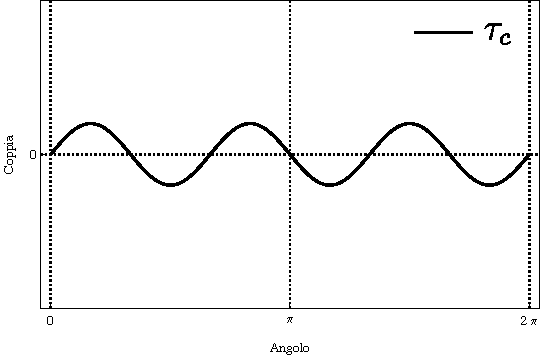
\includegraphics{assets/cogging-torque}
    \caption[Cogging torque]{Cogging toque del motore.}
    \label{fig:cogging}
\end{figure}
